\section{Ejercicio 2}

\subsection{Introducción}

\noindent \underline{\textbf{Contexto}}

En este apartado estamos encarando el diseño de un software de arquitectura, y como parte de este diseño estamos trabajando más específicamente sobre el módulo de Edificios 2D.
Dicho módulo representa a todos los edificios de una ciudad en 2 dimensiones, es decir, en un plano bidimensional. En el plano los edificios son representados por rectángulos apoyados sobre una misma base común. El desafío del proyecto consiste en eliminar las líneas ocultas, dibujando únicamente el horizonte (contorno) que los edificios forman en dicho plano bidimensional.

\noindent \underline{\textbf{El problema a resolver}}

Debemos diseñar un algoritmo que, dado n la cantidad de edificios de un plano, y dados para los n edificios su parante izquierdo, altura y parante derecho, calcule y devuelva el perfil de los n edificios en el horizonte, es decir, el contorno que estos forman en conjunto.
Este contorno debera ser representado a partir de la coordenada en el eje horizontal X de cada punto en donde se produce un cambio de altura, junto con dicha altura.
El problema deberá resolverse en una complejidad temporal estrictamente mejor que O(n$^2$), y deberá poder resolver muchas instancias de planos ingresadas.

\noindent \underline{\textbf{Ejemplos}}

\noindent Para los ejemplos denotaremos:

\textit{N} a la cantidad de edificios del plano bidimensional. \newline
\indent \textit{IZQi} a la coordenada x del parante izquierdo del iésimo edificio. \newline
\indent \textit{ALTi} a la altura del iésimo edificio. \newline
\indent \textit{DERi} a la coordenada x del parante derecho del iésimo edificio.

\begin{enumerate}[leftmargin=0.5cm]
\item N = 4

IZQ1 = 2 ALT1 = 5 DER1 = 6\\
IZQ2 = 3 ALT2 = 2 DER2 = 4\\
IZQ3 = 3 ALT3 = 6 DER3 = 4\\
IZQ4 = 1 ALT4 = 4 DER4 = 5

Contorno resultado: 1 4 2 5 3 6 4 5 6 0

\item N = 5

IZQ1 = 8 ALT1 = 4 DER1 = 9\\
IZQ2 = 6 ALT2 = 4 DER2 = 7\\
IZQ3 = 1 ALT3 = 1 DER2 = 10\\
IZQ3 = 4 ALT3 = 2 DER3 = 8\\
IZQ4 = 2 ALT4 = 5 DER4 = 3

Contorno resultado: 1 1 2 5 3 1 4 2 6 4 7 2 8 4 9 1 10 0

\item N = 5

IZQ1 = 1 ALT1 = 2 DER1 = 3\\
IZQ2 = 2 ALT2 = 2 DER2 = 4\\
IZQ3 = 3 ALT3 = 2 DER2 = 5\\
IZQ3 = 4 ALT3 = 2 DER3 = 6\\
IZQ4 = 2 ALT4 = 2 DER4 = 5

Contorno resultado: 1 2 6 0
\end{enumerate}
\newpage
\subsection{Desarrollo}
Para resolver este problema se analizo que los edificios se podrian llegar a tratar como horizontes individuales, ya que en el caso mas trivial, un edificio es un horizonte. Para mayor legibilidad, en el codigo y pseudocodigo desarrollados, se definieron los siguientes tipos, ademas del tipo ya conocido de edificios:

\begin{itemize}
\item[•]Horizontes es un vector de Horizonte
\item[•]Horizonte es un vector de Coordenada
\item[•]Coordenada es una tupla(x, y) en un plano
\end{itemize}
\bigskip
\noindent \underline{\textbf{Transformacion de Edificios a Horizontes}}

Entonces en primera instancia se transforman los edificios en horizontes con sus coordenadas respectivas: siendo (x1, y, x2) los valores que representan un edificio, realiza una transformacion a dos coordenadas (x1, y)(x2, 0), notar que estas coordenadas siempre estan ordenadas de menor a mayor respecto del eje horizontal X. 

\begin{lstlisting}
Horizontes EdificiosAHorizontes(edificios)
	Para cada edificio i en edificios
		horizontes[i][0].x <- edificio.x1
		horizontes[i][0].y <- edificio.y
		horizontes[i][1].x <- edificio.x2
		horizontes[i][1].y <- 0
	return horizontes
Fin	
\end{lstlisting}

Una vez hecho esto, el problema radicaria en como unir los horizontes. Esto se desglosa en dos sub problemas a resolver:

\begin{enumerate}
\item Como unir dos horizontes.
\item Sabiendo el anterior, que tecnica usar para unir varios de ellos.
\end{enumerate}
\bigskip
\noindent \underline{\textbf{Tecnica para unir varios horizontes}}

Enfocar al problema desde este punto de vista es pensarlo desde una perspectiva \textbf{Divide \& Conquer}, donde los casos base son: hay 1 horizonte, donde se devuelve el mismo, y hay 2 horizontes, en el cual se unen los dos. Para mas de dos horizontes se llama recursivamente con una mitad y la otra, y se los une:

\begin{lstlisting}
Horizonte UnirHorizontes(horizontes, inicio, fin)
	Si fin - inicio == 0
		//Hay un horizonte en horizontes
		return horizontes[inicio]
	Si no
	Si fin - inicio == 1
		//Hay dos horizonte en horizontes
		return Unir(horizontes[inicio], horizontes[fin])
	Si no
	Si fin - inicio > 1
		//Hay mas de dos horizonte en horizontes
		mitad <- [(fin-inicio)/2] + inicio
		return Unir(UnirHorizontes(horizontes, inicio, mitad), UnirHorizontes(horizontes, mitad+1, fin))
Fin	
\end{lstlisting}

\newpage
\noindent \underline{\textbf{Tecnica para unir dos horizontes}}

Ahora queda definir la estrategia para unir dos horizontes. La clave en este punto es tomar la aparicion de cada coordenada como una variacion en la altura, y al momento de analizar que hacer con ella, solamente tener que revisar la relacion con la ultima coordenada analizada del horizonte opuesto. Dicha relacion puede ser mayor, menor o igual en altura. 

Se itera este este procedimiento con cada coordenada de ambos horizontes, siempre eligiendo la coordenada que aparece primero en el eje X para el analisis, y \textbf{manteniendo un invariante} en el que \textbf{las coordenadas en el resultado son el contorno parcial del horizonte final hasta ese momento}.

Una vez que termino de recorrer todo un horizonte, se agregan a continuacion todas las del otro. Esto es debido a que si termino de recorrer uno, significa que la ultima de sus coordenadas aparecia antes que las del contrario, por lo tanto estas ultimas van a formar parte del horizonte resultado.
\bigskip
\begin{lstlisting}
Horizonte Unir(h1, h2)
	Horizonte resultado
	Coordenada ulth1 <- ultima coordenada analizada de h1
	Coordenada ulth2 <- ultima coordenada analizada de h2
	i = 0, j = 0

	Mientras i < h1.size() o j < h2.size() //falta recorrer h1 o h2
		Coordenada actualh1 <- h1[i]
		Coordenada actualh2 <- h2[j]
		
		Si i >= h1.size() //ya se recorrio todo h1
			resultado.agregar(actualh2)
			j++
		Si no
		Si j >= h2.size() //ya se recorrio todo h2
			resultado.agregar(actualh1)
			i++
		Si no
		
		Si actualh1.x < actualh2.x
			Si actualh1.y > ulth2.y
				resultado.agregar(actualh1)
			Si actualh1.y <= ulth2.y
				Si ulth1.y > ulth2.y
					Coordenada auxiliar(actualh1.x, ulth2.y)
					resultado.agregar(auxiliar)
			Si actualh1.y == 0 y ulth2.y == 0
				resultado.agregar(actualh1)
			ulth1 <- actualh1
			i++
		Si no		
		Si actualh1.x > actualh2.x
			Caso analogo al anterior
		Si no		
		Si actualh1.x == actualh2.x
			resultado.agregar(mayorAltura(actualh1, actualh2))
			ulth1 <- actualh1
			i++
			ulth2 <- actualh2
			j++
			
	Fin Mientras
	
	return resultado
Fin	
\end{lstlisting}

%Notar que este pseudocodigo esta hecho con fines practicos para desambiguar la explicacion y entender el analisis hecho para cada coordenada, para mas detalle, ver el codigo de la implementacion.

\newpage
\subsection{Correctitud}

\noindent \underline{\textbf{EdificiosAHorizontes}}

Esta es la primer funcion que se llama al principio de todo el algoritmo, sirve para transformar los edificios que se reciben, a un tipo de dato mas facil de manipular para las funciones que le siguen y ademas asegurar ciertas precondiciones: el contenido de todo horizonte tiene estrictamente dos coordenadas, y estas a su vez estan ordenadas de menor a mayor. Se puede ver facilmente esto en el desarrollo, ya que x1 y x2, representando el parante izquierdo y derecho respectivos de un edificio, siempre se cumple que x1 $<$ x2.

\noindent \underline{\textbf{UnirHorizontes}}

Esta funcion usa la tecnica algoritmica Divide \& Conquer para distribuir la union de los horizontes. Se llama recursivamente: Utiliza un calculo de indices para poder usar una referencia al contenedor de horizontes, evitando asi la copia en cada llamado recursivo. Dichos indices sirven para marcar que horizontes analizar, y siempre se le pasa la mitad del tamaño original, por lo tanto siempre disminuye y va a llegar a un caso base obligatoriamente, que es cuando hay un solo horizonte, o hay dos.

Como nucleo el algoritmo se basa en la funcion Unir, que es la que se encarga de efectivamente unir a a dos horizontes en uno solo.

\noindent \underline{\textbf{Unir}}

Aca queremos probar, que efectivamente la funcion Unir une dos horizontes en uno solo, formando el contorno resultado entre ambos. Para esto se va a utilizar un \textbf{invariante} de ciclo: 

\bigskip
\textbf{Llamaremos a partir de ahora:}
\begin{itemize}
\item[•]H1 y H2 a ambos horizontes respectivos que recibe por parametro, 
\item[•]i y j a los indices de hasta que posicion se recorrio de H1 y H2 respectivamente.
\item[•]Hres al horizonte resultado, en el que se van a ir acumulando el resultado de los analisis entre las coordenadas de H1 y H2
\item[•]actualh1 y actualh2 a las coordenadas actuales respectivas que se analizan de H1 y H2
\item[•]ulth1 y ulth2 a las ultimas coordenadas analizadas de H1 y H2 respectivamente
\item[•]intervalo a la altura que hay entre una posicion x de una coordenada y la siguiente, en la cual se produce un cambio de altura
\item[•]I al invariante
\item[•]B a la guarda del ciclo: i $<$ h1.size() $\vert\vert$ j $<$ h2.size()
\end{itemize}
\bigskip
\textbf{Invariante del ciclo:} 
\begin{itemize}
\item[I1.] Hres esta ordenado desde la posicion 0 hasta i+j de menor a mayor segun el eje x de cada coordenada
\item[I2.] $\forall$intervalo $\in$ Hres, intervalo == mayor intervalo en esa posicion entre H1 y H2.
\item[I3.] $\forall$c1: coordenada $\in$ Hres marcan un cambio de altura, es decir, $\not\exists$ c2:coordenada $\in$ Hres tal que c1 esta al lado de c2 y c1.y == c2.y
\end{itemize}
\bigskip
\textbf{Entonces queremos demostrar:}
\begin{itemize}
\item[I.] Al inicio de la funcion vale I
\item[II.] I sigue valiendo al finalizar cada iteracion
\item[III.] Con cada iteracion nos acercamos mas a $\neg$B
\item[IV.] I $\wedge$ $\neg$B $\Rightarrow$ Qc: Se formo el contorno resultado de unir ambos horizontes totalmente
\end{itemize}
\null
\vfill
[1] Se sabe por la funcion \textbf{EdificiosAHorizontes}, que se utiliza al comienzo del algoritmo, que cada uno de los horizontes transformados tienen sus coordenadas ordenadas de menor a mayor por orden de aparicion en el eje horizontal X, y que ademas la ultima coordenada de estos, la altura vale 0. Entonces podemos suponer que las coordenadas que recibe la funcion Unir siempre estan ordenadas, gracias al invariante sabemos que el resultado va a seguir siempre este orden, concluyendo en que todo horizonte esta ordenado.
\newpage
\noindent \textbf{I. Al inicio de la funcion vale el invariante I}

Como al inicio i = 0 y j = 0, $\Rightarrow$ 
\begin{itemize}
\item[I1.] Hres esta ordenado desde la posicion 0 hasta 0 de menor a mayor segun el eje x de cada coordenada
\item[I2.] No hay ningun intervalo, entonces el para todo se hace verdadero
\item[I3.] No hay ninguna coordenada, entonces el para todo se hace verdadero
\end{itemize}
Entonces vale el invariante porque se cumplieron todas las condiciones de el.\\

\noindent \textbf{II. El invariante I sigue valiendo al finalizar cada iteracion}


Existen cinco casos a analizar\\
\begin{enumerate}
\item \textbf{Si i $>$= h1.size:}

Esto implica que no hay mas elementos de h1 que comparar ya que se los termino de recorrer, por lo tanto agrega al actualh2 al resultado y avanza el j. 
\begin{itemize}
\item[I1.] Como actualh2.x va a tener siempre un valor mayor que ulth1.x, porque sino no hubiese terminado de recorrer h1 y por lo tanto no estaria en este caso, entonces se cumple que sigue estando ordenado.
\item[I2.] Como el intervalo de h1 a partir de que termino quedo en 0, el valor de la coordenada en Hres para el intervalo correspondiente de actualh2.x, va a ser actualh2.y. Entonces se sigue cumpliendo que Hres tiene la mayor altura de intervalos de H1 y H2 en todas sus posiciones.
\item[I3.] Como el H1 no tiene mas coordenadas, se van a seguir agregando las coordenadas de H2 y se sabe por la entrada, que esta no tiene ninguna coordenada que tenga otras coordenadas al lado que repitan su altura. 

El unico caso que se puede llegar a dar, es que justo termino de recorrerse H1 y en la siguiente iteracion a Hres se le empiecen a agregar coordenadas de H2, pero como H1 termino, significa que la altura de su ultima coordenada quedo en 0, y se vera en casos mas adelante, que se lo ignora o transforma por la altura que tiene el intervalo H2 en ese punto. Entonces queda imposible que tenga dos coordenadas consecutivas con la misma altura Hres.\\
\end{itemize}
\item \textbf{Si j $>$= h2.size}

Analogo al anterior, con H1 cambiado por H2	\\

\item \textbf{Si actualh1.x $<$ actualh2.x}

Aun no se termino de recorrer ningun horizonte, por lo tanto elejimos al que este primero segun el eje X (por \textbf{[1]} sabemos que estan ordenados, y vamos a estar eligiendo siempre al menor). 

Como la coordenada actual depende unicamente del ultimo cambio en altura que se hizo, es decir, la altura que venia teniendo el intervalo, y debido a que las coordenadas de un mismo horizonte cumplen con el invariante (si llegase a agregar dos coordenadas seguidas del mismo horizonte no tendria problema ya que cumplen que tienen diferentes alturas) entonces solo se debe analizar respecto de la ultima coordenada analizada del horizonte contrario: necesitamos ver si es mayor, menor o igual respecto a su altura.

\begin{enumerate}
\item Si actualh1.y $>$ ulth2.y

Si la coordenada que estoy analizando actualmente, supera en altura al ultimo intervalo que existe, entonces estoy marcando un nuevo intervalo, por lo tanto se agrega esta nueva coordenada.
\item Si actualh1.y $<=$ ulth2.y

Dado que la coordenada que estoy analizando actualmente, es menor igual en altura al intervalo de H2 en ese punto, esto puede significar dos cosas: 
\begin{enumerate}
\item ulth1.y $>$ ulth2.y

El valor del intervalo del horizonte cuya coordenada que estoy analizando, estaba por arriba del intervalo del horizonte contrario y disminuyo hasta quedar por debajo o igual. Entonces la maxima altura a partir de este punto actualh1.x, deberia ser ulth2.y. Se agrega al resultado entonces la coordenada (actualh1.x, ulth2.y).
\item El valor del intervalo del horizonte cuya coordenada que estoy analizando, estaba por debajo o era igual al del intervalo del horizonte contrario y su nueva altura sigue sin superarlo. Entonces lo ignoro ya que no presenta ningun cambio en la altura maxima del intervalo en este punto.
\end{enumerate}


\item Si actualh1.y $==$ 0 \&\& ulth2.y == 0

Si la coordenada que estoy analizando actualmente tiene altura 0, significa que el contorno que se estaba dibujando se acaba de terminar y ademas la altura del intervalo del horizonte opuesto en ese punto es 0, o sea que ya no habia ningun contorno desde su ultima coordenada, entonces lo unico que importa es que el intervalo del horizonte actual, bajo en altura hasta 0, por lo tanto se agrega la coordenada actualh1 al resultado.
\end{enumerate}

Una vez terminado todo este analisis, como en todos los casos se agrego o se ignoro la coordenada actual, se guarda como la ultima que se proceso y se avanza a la siguiente (i++).

Dado que:

\begin{itemize}
\item[I1.] Se demostro que Hres sigue estando ordenado desde la posicion 0 hasta i+j de menor a mayor segun el eje x de cada coordenada, porque elegimos al menor de ambos siempre.
\item[I2.] Por todo el analisis anterior, en el que se revisa caso por caso cual es el intervalo con mayor altura que deberia ir, quedo demostrado que la eleccion de como elegir la coordenada para agregarla al resultado, va a seguir manteniendo la propiedad en la que el intervalo que marca la nueva coordenada es la mayor altura para ese intervalo en esa posicion entre H1 y H2
\item[I3.] Es imposible que se repita la altura que venia teniendo el intervalo, porque de suceder esto, habria estado repetida tambien en H1, y esto no sucede nunca. Ademas, en el caso que la altura que queriamos agregar ya era <= al intervalo de la ultima coordenada de H2, la ignoramos. Por lo tanto, todas las coordenadas que se encuentran una al lado de otra, marcan diferentes alturas.
\end{itemize}

Entonces quedaron demostradas todas las propiedades, probando que \textbf{se sigue cumpliendo el invariante}.\\

\item \textbf{Si actualh1.x $>$ actualh2.x}

Segundo caso a darse, que la primer coordenada en aparecer no sea la de H1, sino la de H2, es analogo al caso anterior\\

\item \textbf{Si actualh1.x $==$ actualh2.x}

Es el ultimo caso a analizar, en el que ambas aparecen en el mismo momento, entonces la desicion a tomar es elegir la que tiene mayor altura, que va a ser la que marca el intervalo mas alto desde ese punto, por lo tanto se guarda en el resultado la que mayor altura tiene, se guardan ambas coordenadas como las ultimas procesadas, y se avanzan a las siguientes. 

Dado que:

\begin{itemize}
\item[I1.] Se demostro que Hres sigue estando ordenado desde la posicion 0 hasta i+j de menor a mayor segun el eje x de cada coordenada, por \textbf{[1]} siempre se elige a la primer coordenada de cada horizonte, y en este caso ambas aparecen en el mismo momento sobre el eje x, por lo tanto coincide en ambos horizontes, y es la siguiente en orden de aparicion para estar en Hres.
\item[I2.] Quedo comprobado que el intervalo que marca la nueva coordenada es la mayor altura para ese intervalo en esa posicion entre H1 y H2
\item[I3.] Es imposible que se repita la altura que venia teniendo el intervalo, porque de suceder esto, habria estado repetida tambien en H1 o H2, y esto no sucede nunca. Por lo tanto no existe una coordenada en Hres que tenga al lado otra con la misma altura
\end{itemize}
Entonces quedaron demostradas todas las propiedades, probando que \textbf{se sigue cumpliendo el invariante}.
\end{enumerate}
\newpage
\noindent \textbf{III. Con cada iteracion nos acercamos mas a $\neg$B}

En el pseudocodigo se puede observar que hay 3 casos que abarcan toda la iteracion:
\begin{enumerate}
\item Si actualh1.x $<$ actualh2.x $\Rightarrow$ Se incrementa i
\item Si actualh1.x $>$ actualh2.x $\Rightarrow$ Se incrementa j
\item Si actualh1.x == actualh2.x $\Rightarrow$ Se incrementa i y j
\end{enumerate}

B == i $<$ h1.size $\vert\vert$ j $<$ h2.size. 

Se sabe que h1.size y h2.size son fijos y siempre son mayores o iguales a 0, y ademas \textbf{siempre se va a estar incrementando alguna de las variables} i o j, que arrancan desde 0. Entonces por cada iteracion siempre se va a estar acercando cada vez mas al valor de h1.size o h2.size.

Una vez que i alcanza el tamaño de h1.size, esto significa que finalizo de recorrer h1, entonces pasaria a agregar solamente elementos de h2 y a avanzar j. Lo mismo sucede si finaliza de recorrer h2 antes, agrega solamente elementos de h1 y a avanzar i. En el caso de que ambos valores llegan simultaneamente a h1.size y h2.size, entonces ya cumplimos $\neg$B.
\bigskip

\noindent \textbf{IV. I $\wedge$ $\neg$B $\Rightarrow$ Qc }

$\neg$B $\Rightarrow$ i == h1.size \&\& j == h2.size

\textbf{Haciendo reemplazo en de i y j, obtenemos:}

\begin{itemize}
\item[I1.] Hres esta ordenado desde la posicion 0 hasta h1.size + h2.size de menor a mayor segun el eje x de cada coordenada
\item[I2.]  $\forall$intervalo $\in$ Hres, intervalo == mayor intervalo en esa posicion entre H1 y H2.
\item[I3.]  $\forall$c1: coordenada $\in$ Hres marcan un cambio de altura, es decir, $\not\exists$ c2:coordenada $\in$ Hres tal que c1 esta al lado de c2 y c1.y == c2.y
\end{itemize}

Lo cual significa que tenemos el resultado del contorno completo de unir h1 y h2.\nopagebreak

\bigskip
Dado que tenemos \textbf{demostrada la correctitud del ciclo}, sabemos que vale Qc: Se formo el contorno resultado de unir ambos horizontes totalmente. 

Sabemos la funcion Unir cumple la precondicion de i = 0 y j = 0, y realiza el ciclo previamente demostrado, \textbf{Entonces sabemos que la funcion Unir resuelve correctamente la union de dos horizontes.}

La funcion UnirHorizontes para resolver el problema correctamente depende de Unir para unir sus casos recursivos, como demostramos que Unir es correcto, y ademas que UnirHorizontes siempre llega a un caso base, \textbf{queda demostrado que UnirHorizontes es correcto}.
\bigskip

\noindent \underline{\textbf{Correctitud de todo el algoritmo:}}

El algoritmo principal se encarga de ejecutar dos cosas:
\begin{enumerate}
\item La transformacion de EdificiosAHorizontes: se encarga de cumplir las precondiciones de entrada para UnirHorizontes, que los necesita para pasarselos a Unir
\item UnirHorizontes con todos los horizontes que se transformaron anteriormente
\end{enumerate}

Dado que se cumplen los prerrequisitos antes de llamar a UnirHorizontes, y que UnirHorizontes es correcto debido a que Unir es correcto, \textbf{entonces sabemos que el algoritmo en su totalidad es correcto.}

\newpage
\subsection{Complejidad}
Para demostrar la complejidad de este algoritmo, vamos a proceder a analizar por separado las 3 funciones que se utilizan:
\begin{enumerate}
\bigskip
\item \textbf{EdificiosAHorizontes}, se usa al principio del algoritmo, dado que la transformacion de un edificio a horizonte, tiene complejidad constante $\Theta$\textit{(1)}, entonces hacerlo para n edificios tiene costo de \textbf{$\Theta$\textit{(n)}}\bigskip
\item \textbf{Unir} recibe dos Horizonte, que son contenedores de Coordenada, y va iterando sobre cada una hasta haber analizado que hacer con todas las coordenadas, dicho analisis tiene costo $\Theta$\textit{(1)}. Llamemos \textit{c1} y \textit{c2} a la cantidad de coordenadas de cada horizonte respectivamente, realizar entonces el analisis sobre todas las coordenadas tiene una complejidad final de \textit{O(c1 + c2)}, pero como al comienzo del algoritmo siempre se le pide reservar memoria al contenedor para poder almacenar todas las coordenadas, esto pasa a ser $\Theta$\textit{(c1 + c2)}.

Si bien este es un analisis con la cantidad de coordenadas y no de edificios, por la transformacion de edificio a horizonte que se hace al comienzo de todo el algoritmo, se puede ver que en realidad un edificio es lo mismo que dos coordenadas. Pero esto solo vale al principio, ya que una vez realizada la union, la cantidad de coordenadas disminuye o se mantiene igual. Por lo tanto la cantidad de coordenadas siempre se mantiene acotada por el doble de la  cantidad de edificios que hubo en esa union.

Llamemos \textit{n1} y \textit{n2} a la cantidad de edificios de cada horizonte respectivamente, y n a cantidad total de edificios de entrada, por la justificacion anterior entonces se puede ver que \textit{$\Theta(c1 + c2)$} $\in$ \textit{$\Theta(2n1 + 2n2)$}, que termina siendo \textit{$\Theta(2n)$} y finalmente, \textit{\textbf{$\Theta$(n)}}
\bigskip
\item \textbf{UnirHorizontes} realiza dos llamados recursivos con la mitad de horizontes en cada lado, el costo de las operaciones que no son recursivas van a ser \textit{f(n)}, que queda dependiendo de la funcion Unir, ya que todas las demas operaciones son $\Theta(1)$. El caso con un solo horizonte, que simplemente lo devuelve, tiene complejidad $\Theta(1)$.

Esto nos deja en condiciones necesarias y suficientes para poder usar el \textbf{Teorema Maestro}, que sirve para resolver recurrencias de la forma:

\bigskip
$T(n) =\begin{cases} \alpha T(n/c) + f(n) & n > 1 \\ \Theta(1) & n = 1 \end{cases}$

\bigskip
Donde: $\alpha$ = 2, c = 2, y \textit{f(n) =  $\Theta(Unir)$ = $\Theta(n)$ = $\Theta(n^{log_{2}2})$}.

\bigskip
Entonces segun el \textbf{Teorema Maestro}, si \textit{f(n) $\in$ $\Theta(n^{log_{2}2})$} $\Rightarrow$ \textbf{\textit{T(n) = $\Theta$(n log n)}}
\end{enumerate}

\bigskip

Sumando entonces las complejidades de \textbf{EdificiosAHorizontes} y \textbf{UnirHorizontes}, la complejidad final del algoritmo es \textbf{$\Theta$\textit{(n)}} + \textbf{$\Theta$\textit{(n log n)}} = \textbf{$\Theta$\textit{(n log n)}}.

\newpage

\subsection{Experimentación}

Para el proceso de experimentación del problema se plantearon distintas pruebas para corroborar que el algoritmo propuesto funcionara correctamente y que la cota de complejidad encontrada y justificada en la sección anterior, en la práctica, se cumpliera.

Al igual que en el ejercicio 1, dado que el CPU de la computadora utilizada para tomar los tiempos no está atendiendo únicamente a nuestro proceso, realizar una sola vez cada prueba podría darnos valores que no son cercanos a los reales. Por lo que para minimizar este margen de error, a cada prueba se la hizo ejecutar un total de 10.000 veces y se tomó el mejor valor. Notar que tomar el mejor valor no es una mala decisión, ya que mientras más chico sea el valor, más cerca estamos del valor real de tiempo que toma el algoritmo para una instancia dada.

En cada prueba se tomaron métricas para la posterior evaluación del algoritmo en la práctica. Notar que la medición no contempla tiempos de entrada/salida de datos, sino que contempla solamente el núcleo del algoritmo.

Se representó la información tomada mediante gráficos 2D que permitan ver de una manera más clara los resultados obtenidos en las pruebas. Estos fueron realizados con el software QitPlot que la cátedra proveyó.

En cuanto a qué casos testear, nuestro algoritmo no presenta casos “border”. Es decir, no tiene un peor/mejor caso, sino que para cualquier instancia de edificios cargada, realizará el mismo procedimiento, tomando \textbf{$\Theta$\textit{(n log n)}}. Ni el tamaño de los edificios, ni su posición en el suelo de la ciudad, ni la posición relativa entre ellos afecta el tiempo de computo del algoritmo, por lo que el único parámetro variable a la hora de realizar pruebas es la \textbf{cantidad} de edificios.

Esto es así ya que el algoritmo que diseñamos, utiliza la estrategia de Divide \& Conquer para su resolución, como fue mencionado en insisos anteriores. Esta técnica va dividiendo el problema en varios sub-problemas, sin importar la relación entre los edificios de la instancia. Por lo que, si suponemos que existiera un mejor/peor caso de entrada, de todas formas este sería fraccionado en sub-problemas más pequeños hasta llegar al caso base, y el formato de entrada original se habría perdido. Por este motivo es que el algoritmo no presenta un peor ni un mejor caso de resolución.

Dicho, eso, se diseñó un programa que dado un numero n de edificios, genera n edificios aleatorios para probar el algoritmo. Para facilitar la tarea de experimentación, dicho programa era capaz de generar más de una instancia aleatoria, con distintas cantidades de edificios (cada una elegida en la interfaz de dicho programa).

Para todos los casos, se eligió una precisión de hasta 0,0001 ms (milisegundos). De ser menor, la notamos como 0.
En todos los casos se pudo comprobar que la práctica refleja lo expuesto en incisos anteriores.

A continuación presentamos el gráfico 2D que refleja las pruebas realizadas. Para cada tamaño se realizaron pruebas con instancias distintas y aleatorias y las diferencias muy sutiles (del orden de los microsegundos). A sí mismo, a cada una de esas distintas instancias experimentadas de cada tamaño, se la hizo ejecutar un total de 10.000 veces por los motivos explicados anteriormente.\\
	\begin{figure}[h]
		\begin{center}
		   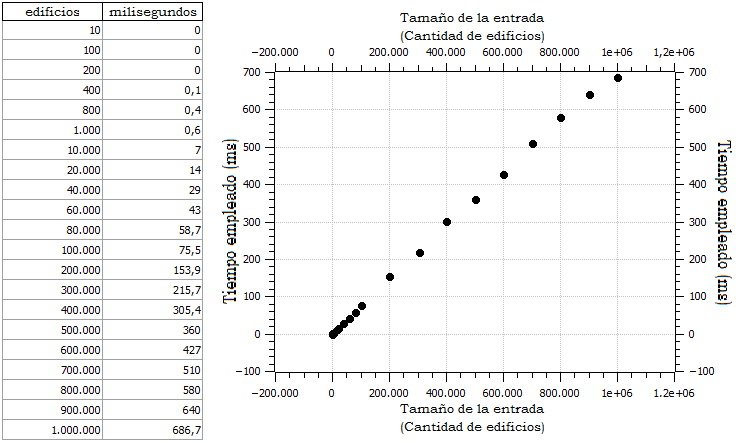
\includegraphics[scale=0.75]{Tests/graficoej2backup.png}
		\end{center}
	\end{figure}